% Pacotes
\documentclass[12pt]{article}
\usepackage{adjustbox}
\usepackage[utf8]{inputenc}
\usepackage{amsmath}
\usepackage{sbc-template}
\usepackage{amsfonts}
\usepackage{fancyvrb}
\usepackage{amsmath}
\usepackage{graphicx,url}


\sloppy

\title{Cálculo da Raiz Quadrada pelo Método de Newton-Raphson\\através do Padrão IEEE-745 para Ponto-Flutuante}

\author{Ricardo Henrique Brunetto\inst{1}}


\address{Departamento de Informática -- Universidade Estadual de Maringá (UEM)\\
	Maringá -- PR -- Brasil
	\email{ra94182@uem.br}
}

\begin{document}

	\maketitle

  \section{Introdução}
	Deseja-se obter uma maneira de estimar a raiz quadrada com base no método iterativo de Newton-Raphson, que
	estimativa de raízes de polinômios e equações transcedentais através da expansão da Série de McLaurin-Taylor.

	Tal método permite obter uma precisão específica através de convergência quadrática (se houver).

	Este artigo fará uma breve explicação do método de Newton-Raphson e do padrão IEEE 754 de armazenamento de ponto-flutuante
	que servirão de base para o desenvolvimento da estratégia utilizada. Não serão feitas explanações a respeito da Série de Taylor-McLaurin,
	visto que foge ao foco do artigo.

	\section{Fundamentação Teórica}
	\label{sec:fund_teor}
	Aqui serão abordados dois tópicos principais em que se baseará o cálculo da raiz quadrada posteriormente na Seção 3:
	o método de Newton-Raphson e o padrão IEEE 754.

	\subsection{Método de Newton-Raphson para determinação de raízes}
	O Método de Newton-Raphson se aplica aos polinômios e às equações transcedentais
	para determinar soluções de sistemas de equações simultâneas, com várias variáveis.
	No escopo deste artigo, seu uso será restringido para determinação de raízes em
	equações polinomiais com uma única variável e, portanto, será feito um breve resumo
	a respeito de seu funcionamento.

	O método de Newton-Raphson se principia com uma raiz aproximada, $x_k$, de uma equação
	$f(x) = 0$, e se vale da expansão em série de Taylor para formular um algoritmo computacional que define uma fórmula
	de recursão para uso.

	O desenvolvimento em série de Taylor de uma função nas vizinhanças do ponto $x_k$ tem a forma
	$$f(x) \approx f(x_k) + f'(x_k)(x - x_k)$$

	onde $f'(X_i)$ indica a derivada primeira de $f(x_k)$ calculada no ponto $(x_k, f(x_k))$.

	Dessa forma, dispõe-se da reta tangente ao gráfico da função $f(x)$, traçada no ponto $x_k$, para deteminação da próxima
	estimativa. Nota-se, que, ao admitir que a função $f(x)$ aproxima-se de sua(s) raiz(es), ocorre $f(x) = 0$ e, portanto, da equação acima:
	$$f(x_k) + f'(x_k) (x-x_k) = 0$$

	Alternativamente, pode-se expressar tal equação como sendo:
	$$f'(x_k) = \frac{f(x_k)}{x_k - x}$$

	Admitindo $x$ como a próxima estimativa, sendo esta mais satisfatória que $x_k$, tem-se a seguinte equação de recorrência, que caracteriza o Método de Newton-Raphson:
	$$x_{k+1} = x_k - \frac{f(x_k)}{f'(x_k)}\;\;\;\;\;\;(1)$$

	\subsection{Padrão IEEE 754}

	Aqui será realizada uma curta abordagem ao padrão IEEE 754 para armazenamento e aritmética binária. Não serão realizadas considerações
	a respeito da quantidade de bits nos diferentes tipos de precisão que o padrão oferece. Nesse caso, o foco torna-se especificamente a
	maneira como os números são acomodados na máquina para entendimento de como se pode manipular esta estrutura a fim de obter cálculos mais rápidos e precisos.

	Qualquer número $x$ pode ser representado por $x = mb^t$, onde $m$ é a mantissa, $b$ é a base e $t$ é o expoente.

	Um número decimal $x$ está representado no padrão IEEE 754 da seguinte forma:
	$$x_{10} = (-1)^{S_2}(1 + M_{10})2^{E_{10} - 1023}$$

	onde:
	\begin{itemize}
		\item $R_b$ implica que $R$ está na base $b$;
		\item $S$ é o valor do bit do sinal;
		\item $M$ é o valor da soma dos bits da mantissa;
		\item $E$ é o valor do expoente (onde $E\in\mathbb{N}$, pois é enviasado);
		\item $1023$ refere-se ao \textbf{BIAS} supondo 11 bits de precisão do expoente.
 	\end{itemize}

	A estrutura permite trabalhar com mantissa $M_2$ (supondo $m$ bits de precisão) de duas formas: inteira ($v_z(M) \in \mathbb{N}$) ou fracionada ($v_f(M) \in \mathbb{R}$).
	$$v_z(M) = \sum_{k=0}^{m-1}{M_b2^{b}}$$
	$$v_f(M) = \sum_{k=1}^{m}{M_k2^{-k}}$$

	onde $b$ e $k$ indexam o "vetor" de bits da mantissa conforme ilustra a figura abaixo.
	\begin{figure}[h]
		\centering
		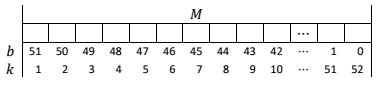
\includegraphics{index_mant}
		\caption{Indexação da mantissa}
		\label{fig:index_mant}
	\end{figure}

	Salienta-se que, de qualquer forma, $v_z(M) = v_f(M)$.

	Assim, passam a existir duas maneiras de se trabalhar com a recuperação do valor armazenado:
	$$x = (-1)^{S}(1 + v_f(M))2^{E - 1023}$$
	ou
	$$x = (-1)^{S}(1 + \frac{v_z(M)}{2^m})2^{E - 1023}$$

	\section{Desenvolvimento}
	\label{sec:desenvolvimento}

	Deseja-se, nesta etapa, desenvolver um método para aplicar Newton-Raphson aproveitando-se do padrão IEEE 754 para calcular a raiz quadrada de um número $A$ em base $10$.

	Sabe-se que
	$$x = \sqrt{A} \implies x^2 = A\\\implies f(x) = x^2 - A = 0$$

	Nota-se que encontrar a raiz quadrada de $A$ significa encontrar o zero da função $f(x)$. Para tal utilizar-se-á Newton-Raphson.

	Da Seção 2.2, sabe-se que $A = m_a2^{e_a}$. Da mesma forma, $x = m_x2^{e_x}$.

	Ao aplicar Newton-Raphson em $f(x)$, tendo $x_k$ como estimativa inicial, tem-se:
	$$x_{k+1} = x_k - \frac{x_k^2 - A}{2x_k}$$
	que pode ser reescrito como:
	$$x_{k+1} = \frac{3x_k - x_k^2 + A}{2x_k}$$
	$$\equiv x_{k+1} = \frac{3x_k}{2x_k} - \frac{x_k^2}{2x_k} + \frac{A}{2x_k}$$
	$$\equiv x_{k+1} = \frac{3}{2} - \frac{x_k}{2} + \frac{A}{2x_k}$$
	$$\equiv x_{k+1} = 1.5 - \frac{x_k}{2} + \frac{A}{2x_k}$$

	Nota-se que $x_k = m_{x_k}2^{e_{x_k}}$ no padrão IEEE 754. Portanto,

	$$x_{k+1} = 1.5 - m_{x_k}2^{e_{x_k} - 1} + \frac{A}{m_{x_k}2^{e_{x_k} +1}}$$
	$$\equiv x_{k+1} = 1.5 - m_{x_k}2^{e_{x_k} - 1} + \frac{m_a2^{e_a}}{m_{x_k}2^{e_{x_k} +1}}$$
	$$\equiv x_{k+1} = 1.5 - m_{x_k}2^{e_{x_k} - 1} + \frac{m_a}{m_{x_k}}2^{e_a - e_{x_k} + 1}$$

	Adotando a extração fracionária do valor da mantissa, tem-se:
	$$x_{k+1} = 1.5 - m_{x_k}2^{e_{x_k} - 1} + \frac{m_a}{m_{x_k}}2^{e_a - e_{x_k} + 1}$$

	Nota-se que $\frac{m_a}{m_{x_k}}$ pode ser escrito como
	$$\frac{v_f(m_a)}{v_f(m_{x_k})}$$

	Substituindo $x_k$ por $x_i$:
	$$\frac{v_f(m_a)}{v_f(m_{x_i})} = \frac{\sum_{k=1}^{m}{(M_a)_k2^{-k}}}{\sum_{k=1}^{m}{({M_{x_i})_k2^{-k}}}}$$

	Note que a soma e subtração nos expoentes podem ser feitas com \textit{bit shift}.

	\section{Conclusão}
	$$x_{k+1} = 1.5 - m_{x_k}2^{e_{x_k} - 1} + \frac{m_a}{m_{x_k}}2^{e_a - e_{x_k} + 1}$$

	Dessa forma, conclui-se que é possível aplicar Newton-Raphson onde cada iteração necessita de:
	\begin{itemize}
		\item 2 subtrações
		\item 1 adição
		\item 2 bit-shifts
		\item 1 divisão
	\end{itemize}

	Provavelmente é possível executar melhoras nesta técnica, porém, necessita de um estudo mais aprofundado.

\end{document}
